%\documentclass[12pt]{article}
\documentclass[12pt]{book} % for chapters
%\usepackage{fullpage}
%\usepackage[top=1in,bottom=1in,left=1in,right=1in]{geometry}
\usepackage[margin=1in, paperwidth=8.5in, paperheight=11in]{geometry}
\usepackage[english]{babel}
\usepackage[utf8x]{inputenc}
\usepackage{amsmath}
\usepackage{graphicx}
\usepackage{caption}
\usepackage[depth=subsection]{bookmark}
\usepackage{multirow}
\usepackage[usestackEOL]{stackengine}
%https://www.sharelatex.com/learn/Code_listing
%For code view in latex

\usepackage{pdflscape}

\usepackage{listings}


%\usepackage[linktocpage=true]{hyperref}
\hypersetup{
    pdfborder = {0 0 0}
}

\usepackage[colorinlistoftodos]{todonotes}
\usepackage{chngcntr}
\usepackage{url}
%header and footer package
\usepackage{fancyhdr}
\usepackage[en-US]{datetime2}
\usepackage{adjustbox}


\usepackage{booktabs}
\usepackage{xcolor}
\usepackage{colortbl}



%clearing default page heading and footer
\pagestyle{fancy}



\fancyhf{}
%
\ifx
     E for even page
    O for odd page
    L for left side
    C for centered
    R for right side 
\fi
\lfoot{\fancyfoot[LE,LO]{\leftmark}} 
\rfoot{ PAGE - \thepage} 



\fancyhead{}
\renewcommand{\footrulewidth}{1pt}
\renewcommand{\headrulewidth}{0pt}
\parindent 0ex
\renewcommand{\baselinestretch}{1.5}

% Redefine the plain page style
\fancypagestyle{plain}{%
    \lfoot{\fancyfoot[LE,LO]{\leftmark}} 
    \rfoot{ PAGE - \thepage} 
}




\begin{document}


\begin{titlepage}

\newcommand{\HRule}{\rule{\linewidth}{0.5mm}} % Defines a new command for the horizontal lines, change thickness here
\center % Center everything on the page
 
%----------------------------------------------------------------------------------------
%	HEADING SECTIONS
%----------------------------------------------------------------------------------------

\textsc{\Large Department of Computer Science \& Engineering}\\[0.5cm] % Name of your university/college
\textsc{\Huge United International University}\\[1cm] % Name of your university/college
 %\textsc{\Large Major Heading}\\[0.5cm] % Major heading such as course name
 % \textsc{\large Minor Heading}\\[0.5cm] % Minor heading such as course title

%----------------------------------------------------------------------------------------
%	TITLE SECTION
%----------------------------------------------------------------------------------------

\HRule \\[0.4cm]
{ \huge \LARGE \textbf{CSE6011: Data Mining}}\\ [0.4cm] % Title of your document
{ {\Large \textbf{Forecasting SMS Traffic and Balance Availability with Machine Learning}}}\\
\HRule \\ [1cm]
%  \textit{A dissertation submitted to the United International University in partial fulfillment of the
% requirement for the degree B. Sc. in Computer Science \& Engineering}
%----------------------------------------------------------------------------------------
%	AUTHOR SECTION
%----------------------------------------------------------------------------------------


\begin{minipage}{0.5\textwidth}
\begin{flushleft} \small
\emph{\textbf{\large Author}:}\\
Mohammad Saifur Rahman  \\ % Your name
ID : 0122420002\\
Nirupom Das Dipto  \\ % Your name
ID : 0122230023\\
Md Mizanur Rahman \\ % Your name
ID : 0122420016\\
Md. Raqibur Rahman  \\ % Your name
ID : 0122310001\\

\end{flushleft}
\end{minipage}
~
\begin{minipage}{0.4\textwidth}
\begin{flushright} \large
\emph{\textbf{Supervisor}:} \\
Dr. Mohammad Nurul Huda  \\% Supervisor's Name
Professor, Head of CSE Dept. \\
Department of CSE, UIU\\

\end{flushright}
\end{minipage}\\[3cm]

% If you don't want a supervisor, uncomment the two lines below and remove the section above
%\Large \emph{Author:}\\
%John \textsc{Smith}\\[3cm] % Your name

%----------------------------------------------------------------------------------------
%	DATE SECTION
%----------------------------------------------------------------------------------------

\ifx
\textregistered\textcopyright
\sffamily\textregistered\textcopyright
\fi

Copyright\textcopyright{Year \the\year}\\
%{\large \today}\\[2cm] % Date, change the \today to a set date if you want to be precise
\DTMlangsetup{showdayofmonth=false}
\today\\[1cm]
%----------------------------------------------------------------------------------------
%	LOGO SECTION
%----------------------------------------------------------------------------------------


\includegraphics[width=100px]{assets/uiu-logo.png}\\[1cm] % Include a department/university logo - this will require the graphicx package
 
%----------------------------------------------------------------------------------------

\vfill % Fill the rest of the page with whitespace

\end{titlepage}


%=========COVER PAGE ENDS HERE==========================
%=========COVER PAGE ENDS HERE==========================



\pagenumbering{roman}




%==================Table of contents PAGE starts HERE=============
%==================Table of contents PAGE starts HERE=============
%\frontmatter
\pagenumbering{arabic}
\counterwithin{equation}{chapter}
% \counterwithin{figure}{chapter}






\thispagestyle{empty}
    \addtocontents{toc}{\protect\thispagestyle{empty}}
\tableofcontents
\thispagestyle{empty}
\clearpage

%\addtocontents{toc}{~\vfill}
\addtocontents{toc}{~\hfill{\large \textbf{Chapters}}}
\addtocontents{toc}{~\hfill{\large \textbf{Page}}\par}

%==================Table of contents PAGE ends HERE=============
%==================Table of contents PAGE ends HERE=============




\setcounter{page}{1}


%=================Introduction PAGE Starts HERE=================
%=================Introduction PAGE Starts HERE=================


\chapter{Introduction}
This report presents a comprehensive analysis of SMS traffic and balance availability for a specific set of clients, with a particular focus on predicting potential service interruptions during holidays. By utilizing advanced machine learning techniques, such as \textbf{polynomial regression}, we aim to accurately forecast future SMS traffic and balance levels, enabling clients to optimize their usage and avoid unexpected service disruptions. 

By using advanced data analytics, this study provides a comprehensive forecast of SMS traffic and balance levels, enabling organizations to proactively manage their client communication strategies and resource allocation. This predictive model accurately anticipates SMS traffic during peak periods, such as holidays, and offers hourly updates on balance levels for the next two days, ensuring a seamless and uninterrupted service experience for clients.

Ultimately, this research contributes to the field of machine learning applications and provides practical solutions for organizations seeking to effectively manage their SMS balance allocation to clients, particularly during peak demand periods like holidays.


%Introduction PAGE ends HERE----------
%Introduction PAGE ends HERE----------




\section{Background}
At Wintel Limited, there was a need for SMS balance forecasting analysis to predict SMS traffic and balance levels in advance. By anticipating these factors, the company can avoid SMS shortages during peak times, such as holidays or unexpected events, ensuring continuous service availability.

\subsection{Objectives​}
\begin{itemize}
    \item The objectives of this project is to develop a predictive model using advanced machine learning techniques to accurately forecast masking and non-masking SMS traffic and balance levels for a specific set of clients. More specifically the purpose of this project is to generate next 2 days predictions.​
    \item To identify potential service interruptions during peak periods, such as holidays, and provide early warnings to organizations and its clients.​
    \item To enable organizations to optimize their SMS communication strategies and resource allocation by providing timely information on SMS traffic and balance levels.​
    \item To contribute to the field of machine learning applications by demonstrating the effectiveness of polynomial regression in predicting SMS traffic and balance.​
    \item To provide practical solutions for organizations seeking to improve their SMS communication infrastructure and deliver exceptional customer service.​
\end{itemize}





\subsection{The Problem}

In today's fast-paced world, SMS communication has become an integral part of our daily lives. For organizations with a large customer base, managing SMS traffic and ensuring adequate balance availability can be a complex challenge, especially during peak periods such as holidays. Service interruptions due to insufficient balance or overloaded networks can lead to customer dissatisfaction and financial losses.

\subsection{The Solution}

To address these challenges, this report presents a comprehensive analysis of SMS traffic and balance prediction \& automation for a specific set of clients. By employing advanced machine learning techniques, such as \textbf{polynomial regression}, we aim to develop a predictive model that can accurately forecast future SMS traffic and balance levels. This information will empower organizations to make informed decisions regarding their communication strategies and resource allocation, ensuring a seamless and uninterrupted service experience for their clients.

\subsection{The Benefits}
\begin{itemize}
		\item \textbf{Improved Service Quality:} Accurate predictions of SMS traffic and balance levels will enable organizations to proactively address potential issues, ensuring a consistent and reliable service experience for their clients.
        \item \textbf{Optimized Resource Allocation:}  By understanding future demand, organizations can allocate resources more efficiently, reducing employees hours of struggle during the holidays and minimizing service disruptions.
        \item \textbf{Enhanced Customer Satisfaction:} A reliable and uninterrupted SMS service can significantly improve customer satisfaction and loyalty.
        \item \textbf{Data-Driven Decision Making:} The insights gained from this analysis will provide organizations with a data-driven foundation for making informed decisions about their SMS communication strategies.
\end{itemize}


This report aims to contribute to the field of machine learning applications and provide practical solutions for organizations seeking to optimize their SMS communication infrastructure and deliver exceptional customer service.




\subsection{Significance of our project}
Forecasting SMS traffic flow using machine learning algorithms offers a powerful method for not only predicting SMS volumes based on historical data but also incorporating various external factors that may affect traffic.

External factors like weather conditions, time of day, and calendar events can introduce irregularities in SMS traffic patterns, making it crucial to account for these variables when building forecasting models.

By integrating these external variables into the prediction model, machine learning algorithms can generate more accurate forecasts. These improved predictions help organizations make more informed decisions about how to manage SMS traffic flows, optimize resource allocation, and improve operational efficiency.




\section{Literature Review}



\section{Research Gap}
\section{Objectives}

\begin{itemize}

    \item The objectives of this paper is to develop a predictive model using advanced machine learning techniques to accurately forecast masking and non-masking SMS traffic and balance levels for a specific set of clients. More specifically the purpose of this project is generate next 2 days predictions.
    \item To identify potential service interruptions during peak periods, such as holidays, and provide early warnings to organizations and it's clients.
    \item To enable organizations to optimize their SMS communication strategies and resource allocation by providing timely information on SMS traffic and balance levels.
    \item To contribute to the field of machine learning applications by demonstrating the effectiveness of polynomial regression in predicting SMS traffic and balance.
    \item To provide practical solutions for organizations seeking to improve their SMS communication infrastructure and deliver exceptional customer service.
\end{itemize}


% Section 1.1: Background

%     Overview of SMS usage and its significance.
%     Brief history of SMS technology.

%     Importance of accurate SMS traffic and balance prediction.

% Section 1.2: Literature Review

%     Existing research on SMS traffic prediction.
%     Review of machine learning techniques used for prediction.
%     Analysis of the limitations of previous studies.

% Section 1.3: Research Gap

%     Identification of the specific gap in the existing research.
%     Explanation of the need for a more comprehensive and accurate prediction model.

% Section 1.4: Objectives

%     Clear statement of the research objectives.
%     Outline of the goals to be achieved


    

\chapter{Methodology}

\section{Corpus Collection}
% Section 2.1: Corpus Collection
%     Description of the data sources used.
%     Explanation of the data collection process.
%     Data preprocessing techniques (cleaning, normalization, etc.).

\subsection{Dataset}

\begin{table}[h!]
    \centering
    \begin{tabular}{|c|c|}
        \hline
        \textbf{Date} & \textbf{Balance} \\ \hline
        2024-09-24 & 138706 \\ \hline
        2024-09-25 & 138214 \\ \hline
        2024-09-26 & 137241 \\ \hline
        2024-09-27 & 134192 \\ \hline
        2024-09-28 & 118229 \\ \hline
        2024-09-29 & 116883 \\ \hline
        2024-09-30 & 113839 \\ \hline
        2024-10-01 & 112638 \\ \hline
        2024-10-02 & 111951 \\ \hline
        2024-10-03 & 110807 \\ \hline
        2024-10-04 & 105434 \\ \hline
        2024-10-05 & 103655 \\ \hline
        2024-10-06 & 100337 \\ \hline
        2024-10-07 & 96591 \\ \hline
        2024-10-08 & 86970 \\ \hline
        2024-10-09 & 162602 \\ \hline
        2024-10-10 & 155813 \\ \hline
        2024-10-11 & 155048 \\ \hline
        2024-10-12 & 154230 \\ \hline
        2024-10-13 & 154108 \\ \hline
    \end{tabular}
    \caption{Balance Data from 2024-09-24 to 2024-10-13}
    \label{tab:balance_data}
\end{table}


\begin{itemize}
    \item \textbf{Total Dataset:} 20 incidents (achieved from the work-data till date)
    \item \textbf{Training Data:} 70\% of the total dataset
    \item \textbf{Testing Data:} 30\% of the total dataset
\end{itemize}

\subsection{Experimental Setup}

\begin{itemize}
    \item \textbf{Polynomial Degree:} We have considered the best-fit degree of 2 for our model.
    \item \textbf{Accuracy Checking:} We have analyzed whether the real-life SMS traffic requirement lies within the predicted SMS traffic values generated by our model.
\end{itemize}



\subsection{Description of the data sources used}
For this project, data from Wintel Limited is used. To achieve better results and improve model building, a real-life, real-time dataset will be used, ensuring more accurate and practical outcomes.

\subsection{Data Collection Process}
In wintel each 4 hours a cron/scheduler will be called where this model will work and generate the predictions. For Both masking and non-masking sms traffic and balance seperate models will be called. In each day approximately 6 times the this process will work. We will pick last 180 days dataset from wintext portal mssql database and use it to the model.

\subsection{Data preprocessing techniques}

\begin{itemize}
    \item Timestamps were converted into a consistent datetime format to facilitate accurate time-series analysis.
    \item SMS traffic counts and balance levels were ensured to be in numeric formats for proper calculation and analysis.
    \item Duplicate records in SMS traffic logs were identified by checking for identical timestamps, client IDs, and traffic counts.
    \item Special care was taken to adjust for traffic and balance patterns during holidays, which often exhibit different behaviors from regular periods. Historical holiday data was cross-referenced with the current dataset to ensure accurate classification and analysis.
    \item  SMS Traffic per Operator \& Client: The SMS traffic per operator and client was calculated to analyze usage patterns.
    \item Balance per Client: The balance per client was calculated to assess balance allocation.
    \item Balance per Operator: The balance per operator was calculated to assess balance allocation to opertor wise.
\end{itemize}


















\subsection{Polynomial Regression}

\textbf{Polynomial Regression} is an extension of linear regression where the relationship between the independent variable(s) and the dependent variable is modeled as an $n$th-degree polynomial. This method is particularly effective when the data exhibit non-linear relationships that cannot be captured by a simple linear regression model.

The general form of a polynomial regression equation is:

\[
y = \beta_0 + \beta_1 x + \beta_2 x^2 + \beta_3 x^3 + \dots + \beta_n x^n + \epsilon
\]

Where:
\begin{itemize}
    \item $y$ is the dependent variable (response variable).
    \item $x$ is the independent variable (predictor variable).
    \item $\beta_0, \beta_1, \dots, \beta_n$ are the coefficients of the polynomial.
    \item $\epsilon$ is the error term (residuals).
\end{itemize}

\subsection{Key Terms in Polynomial Regression}
\begin{itemize}
    \item \textbf{Polynomial Terms}: These are the powers of the independent variable(s), such as $x^2$, $x^3$, etc., that enable the model to fit non-linear data.
    \item \textbf{Degree of Polynomial}: This refers to the highest exponent in the polynomial equation (e.g., $n$ in $x^n$). Higher degrees capture more complexity in the data but can lead to overfitting.
    \item \textbf{Least Squares Method}: The coefficients $\beta_0, \beta_1, \dots, \beta_n$ are estimated by minimizing the sum of squared residuals between the observed and predicted values.
\end{itemize}



\subsection{System Diagram}


\begin{figure}[h]
	\begin{center}
		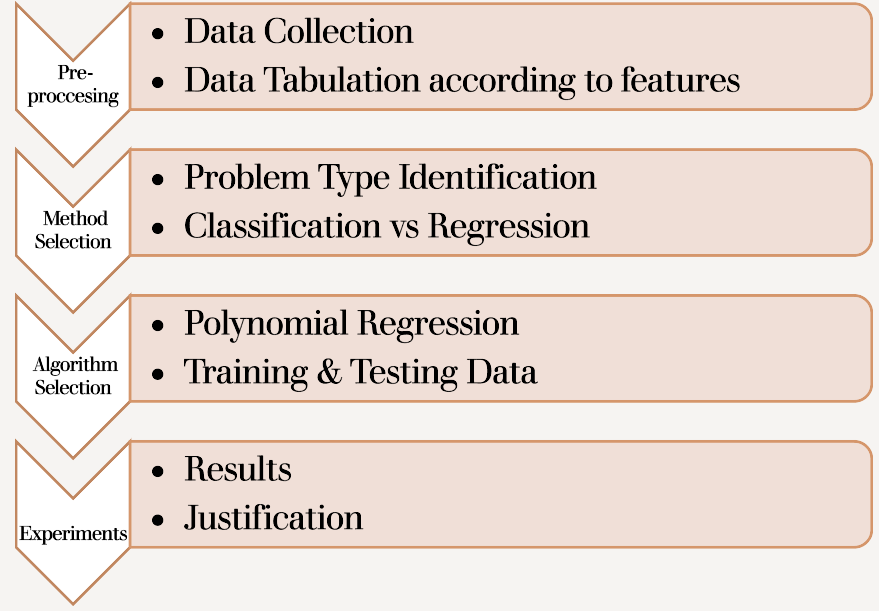
\includegraphics[width=0.5\textwidth]{assets/sysdiagram.png} 
	\end{center}
	\caption{System Diagram} % Use caption* to avoid adding it to the list of figures
	\label{fig:systemdiagram}
\end{figure}





% \subsection{Training Data}

% \subsection{Test Data}


% \subsection{Cross-Validation}
% To avoid overfitting and ensure model generalization, we applied 5-fold cross-validation. The dataset was split into 5 equal parts, with each part used as a test set while the remaining data served as the training set. This process was repeated 5 times, and the average RMSE across all folds was used to evaluate model performance.

% Section 2.2: Training Data
% https://www.youtube.com/watch?v=vAi6bCTFuAY


%     Details of the training dataset.
%     Features selected for training.
%     Data splitting for training and validation.

% Section 2.3: Test Data

%     Description of the test dataset.
%     Evaluation metrics to be used.

% Section 2.4: Experimental Setup

%     Overview of the experimental design.
%     Configuration of the machine learning model.
%     Hyperparameter tuning methodology.


\chapter{Experimental Results and Analysis}
% Section 3.1: Model Performance

%     Presentation of the experimental results.

%     Evaluation of the model's accuracy, precision, recall, and F1-score.
%     Comparison with baseline models or previous studies.

% Section 3.2: Analysis of Findings

%     Discussion of the insights gained from the results.
%     Explanation of the model's strengths and limitations.
%     Identification of any unexpected outcomes.


\section{RESULTS and DISCUSSION}
\subsection{Visualization of Predicted vs. Actual SMS Volumes}

\begin{figure}[h]
	\begin{center}
		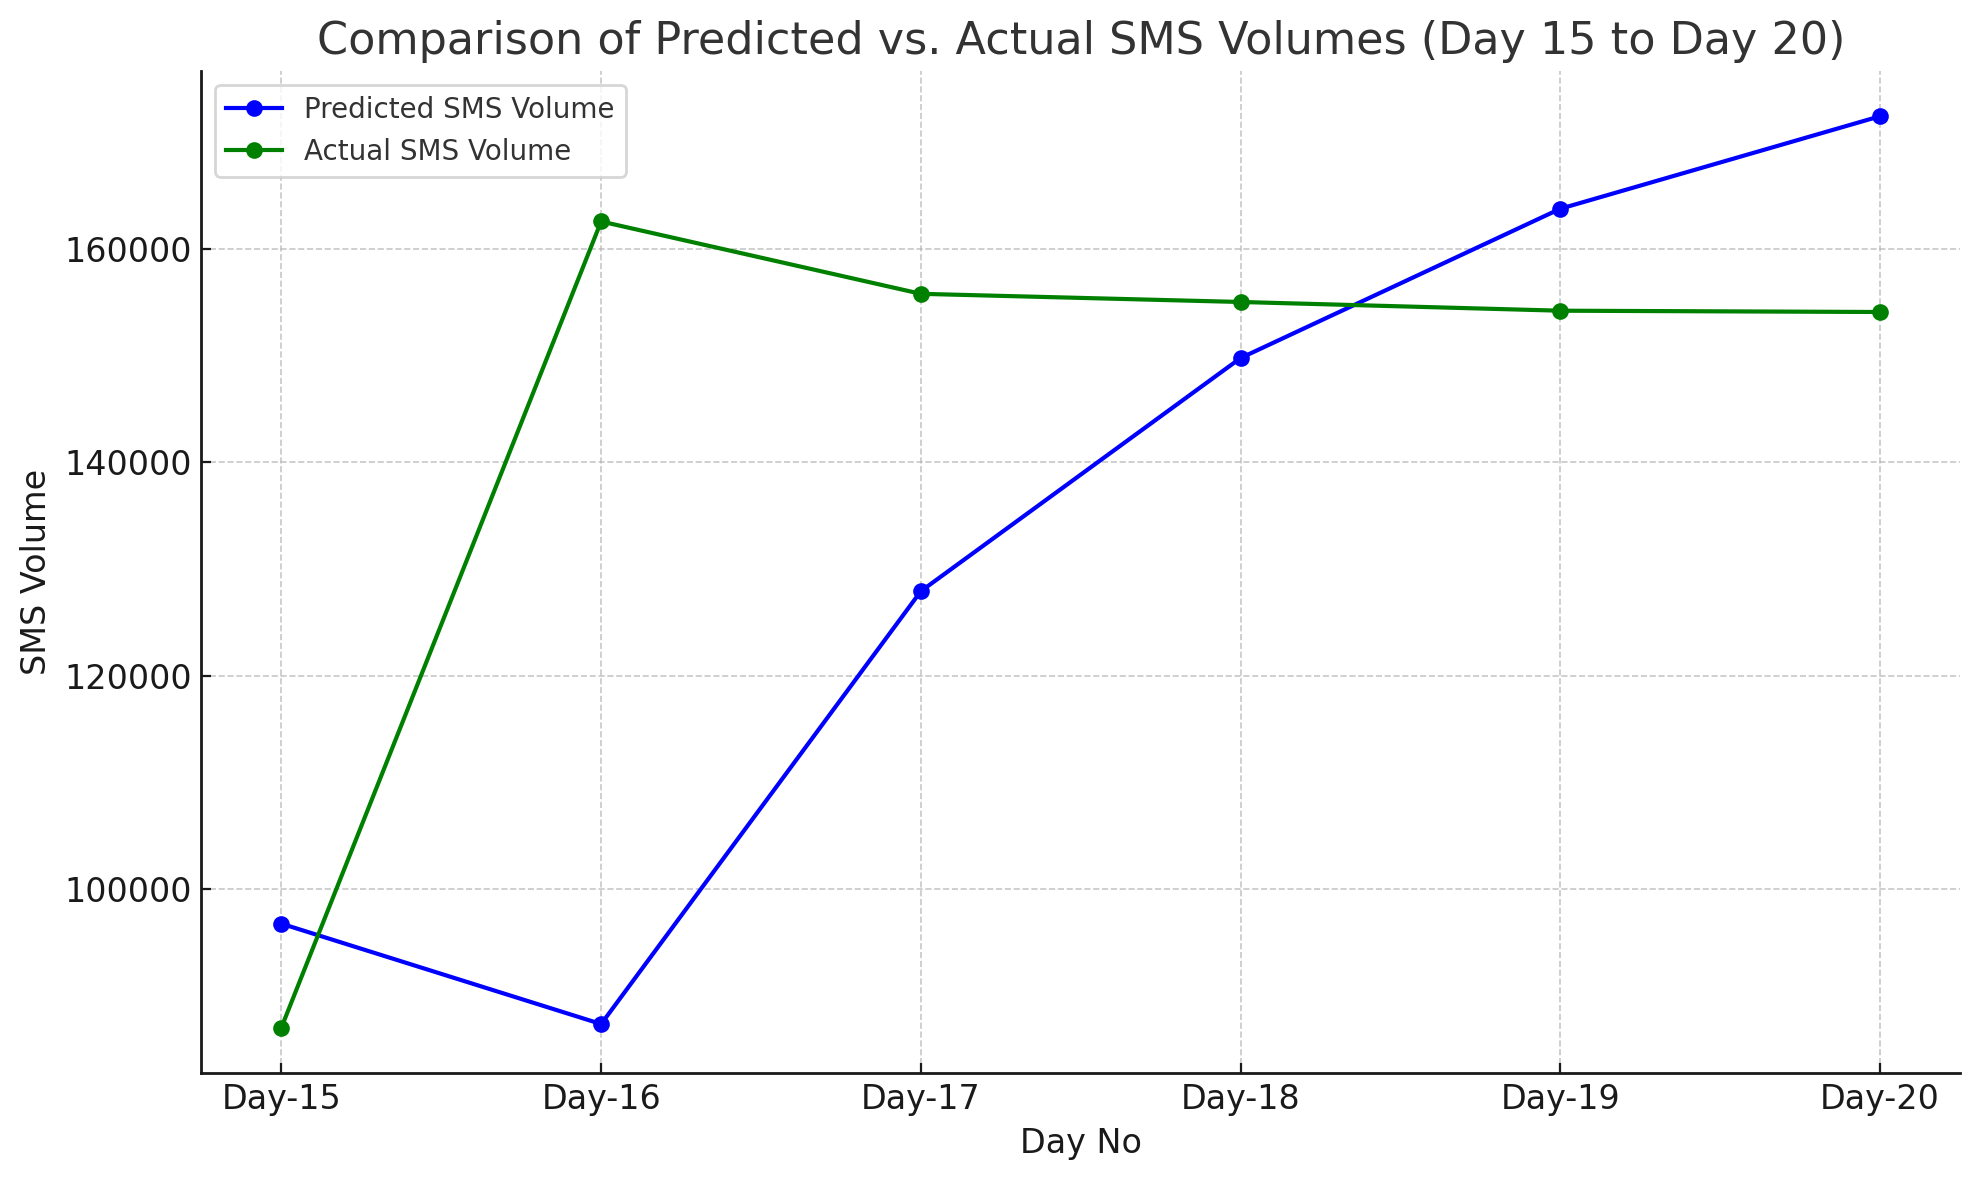
\includegraphics[width=0.8\textwidth]{assets/result-predicted-vs-actual-sms-balance.png} 
	\end{center}
	\caption{Visualization of Predicted vs. Actual SMS Volumes} % Use caption* to avoid adding it to the list of figures
	\label{fig:result-predicted-vs-actual-sms-balance}
\end{figure}


The chart below visualizes the comparison between predicted and actual SMS volumes for Days 15 to 20, along with the error percentage for each day:
Here is the chart that compares the predicted and actual SMS volumes for Days 15 to 20. The blue line represents the predicted SMS volumes, while the green line represents the actual SMS volumes. This visualization clearly highlights where the predictions were close to the actual values and where they diverged.



\begin{table}[ht]
    \centering
    \caption{Comparison of Predicted and Actual SMS Volumes with Accuracy Percentage}
    \begin{adjustbox}{max width=\textwidth}
    \begin{tabular}{|c|c|c|c|c|}
    \hline
    \rowcolor{lightgray} \textbf{Day No} & \textbf{Predicted SMS Volume} & \textbf{Actual SMS Volume} & \textbf{Error Percentage} & \textbf{\% of Accuracy} \\
    \hline
    Day-15 & 96719 & 86970 & 0.112096 & 90\% \\
    \hline
    Day-16 & 87303 & 162602 & -0.463088 & 186\% \\
    \hline
    Day-17 & 127912 & 155813 & -0.179067 & 122\% \\
    \hline
    Day-18 & 149789 & 155048 & -0.033919 & 104\% \\
    \hline
    Day-19 & 163796 & 154230 & 0.062024 & 94\% \\
    \hline
    Day-20 & 172475 & 154108 & 0.119183 & 89\% \\
    \hline
    \end{tabular}
    \end{adjustbox}
    \label{tab:comparison}
\end{table}


\chapter{Conclusion and Future Works}
% Section 4.1: Summary of Findings

%     Recapitulation of the key research findings.

%     Highlights of the contributions made.

% Section 4.2: Limitations

%     Acknowledgment of the study's limitations.
%     Discussion of potential areas for improvement.

% Section 4.3: Future Directions

%     Suggestions for future research.
%     Potential extensions or applications of the work.




\section{Conclusion}

This report presents a comprehensive study on forecasting SMS traffic and balance availability using machine learning techniques. By leveraging historical data from Wintel Limited, we developed a predictive model capable of providing accurate forecasts for SMS traffic and balance levels over the next two days. This model has demonstrated its ability to anticipate potential service interruptions, particularly during holidays and other peak periods, ensuring clients can optimize their SMS usage and avoid disruptions.

Key benefits of this work include:

\begin{itemize}
    \item Improved service reliability during peak traffic periods.
    \item Enhanced resource allocation based on accurate demand forecasts.
    \item Increased customer satisfaction through proactive management of SMS traffic and balances.
\end{itemize}

Overall, this project contributes to the practical application of machine learning in managing communication resources, especially in time-sensitive environments where uninterrupted service is critical.


\section{Future Works}

While the current model demonstrates strong predictive capabilities, several areas for future research and improvement have been identified:

\begin{itemize}
    
    \item \textbf{Model Optimization:} Future iterations of the model can explore the use of advanced machine learning techniques, such as deep learning or ensemble models, to improve prediction accuracy, especially for more complex traffic patterns. Also we don't have currently all 180 days real dataset to actually verify original outcomes. After getting 180 days dataset we can verify the model more accurately.
    \item \textbf{Incorporation of Additional Features:} Additional factors, such as external events, marketing campaigns, or changes in client behavior, can be incorporated into the model to refine its forecasts further.
    \item \textbf{Real-Time Prediction:} While this report focused on hourly predictions, the model can be extended to provide real-time updates, allowing for even more dynamic resource management.
    \item \textbf{Scalability:} Further research is needed to test the scalability of the model across a broader set of clients and operators, particularly for large-scale applications where SMS traffic volume is significantly higher.
    \item \textbf{Exploring Different Algorithms:} Polynomial regression was used for this project, but future work could evaluate the performance of alternative algorithms, such as decision trees, random forests, or gradient boosting methods, to find the best fit for the problem domain.
    \item \textbf{Integration with Automated Systems:} Finally, future work can focus on integrating the predictive model into automated systems that can automatically allocate resources or send alerts to clients when balances are predicted to drop below a critical threshold.
\end{itemize}

By addressing these areas, we can further enhance the reliability and robustness of SMS traffic and balance prediction systems, ultimately improving client experiences and operational efficiency.

\end{document}
